\section{Introduction}
Due to the cognitive burden of memorizing a large number of online credentials, users of the web have resorted to using a limited subset of short and simplistic password pairs that leave accounts vulnerable to exploitation \cite{user_behaviours}.

Cyber threat actors have evolved into formidable opponents, often possessing a wide range of tools and exploits that can be used to compromise password security. The implications are that users need a software solution that manages access to online accounts in a secure manner while reducing the number of credentials that need to be memorized.

Password managers with pseudo single sign on (SSO) capability are one solution to the account management problem. Single sign on technology allows users to log into any of their accounts through a single unified interface.

This paper will explore the development of a USB based password manager system. Credentials will be required to be stored in an encrypted form on a hardware based medium. The system should also be able to decrypt the relevant credentials from file storage and perform the required SSO functionality. The goal is to develop an SSO solution that requires a user to only log into each individual account once before SSO functionality takes effect.

Various challenges to developing a USB based password manager exist, including implementing a suitable USB driver, filesystem and encryption to secure credentials. Additionally various electronics are required to interface with the USB port of a host PC. 

\subsection{Aims}
This report is focused on the overall system design and security analysis of a self-encrypting hardware based password manager. 

The design procedure is expected to be linear with a high level design being followed by a more detailed system level design. This is then followed by various experimentation to evaluate key security objectives.

Namely the aims of this report are to:
\begin{itemize}
  \item Investigate the various requirements (tools) to develop the necessary software and hardware subsystems.
   \item Investigate SSO as well as password managers.
  \item Research common attack vectors that lead to password compromise as well as defenses.
  \item Research password specific algorithmic standards and performance.
  \item Create a working prototype of the overall system from the software and hardware components identified earlier.
  \item Experimentation to determine the overall security objectives of each subsystem.
  \item Analyse the results using qualitative and quantitative methods.
  \item Draw conclusions from the provided data.
  
\end{itemize}

\subsection{Background}
Password confidentiality can be characterised according to the endpoints involved (Figure 1.1) in a security related exchange as well as the data transmission channel. For a self-encrypting USB drive one approach is to have a software client (endpoint 2) run on the end user's computing device. The host USB device (endpoint 1) would then take over the role of encrypting/decrypting user credentials and would communicate with the software client to process commands. Communication could be through a traditional transmission channel such as serial or RS232.

During a request to have a credential encrypted the software client could send the plain-text password over the serial link to the host USB device along with the encryption key. At the host USB end the password is then encrypted with the secret key. An opponent may have access to the data transmission channel during encryption and could theoretically capture sensitive information such as the encryption key or plain-text password. 

The ability of a password manager to function securely is solely dependant on the confidentiality and integrity of the secret key. If the secret key is compromised in any way an opponent may be able to decrypt communication between both endpoints and compromise the corresponding credential. Confidentiality is the ability to prevent unauthorized disclosure of secret information while integrity is the ability to protect data from unauthorized changes\cite{network_security}.

Another possibility is that an opponent prevents the legitimate recipient from encrypting the credential in the first place in what is known as denial of availability or denial of service. Denial of service (DoS) attacks are common and can cause widespread service outages for extended periods of time. These attacks target the availability of data.


Overall four basic tasks exist in designing a password manager system with SSO capabilities:

\begin{itemize}
  \item Choose an algorithm to encrypt/decrypt user credentials. 
  \item Design a secret key generator to be used as part of the encryption algorithm.
  \item Develop a secure method of password storage.
  \item Design a user interface to manage password storage.
  \item Develop a method of automatically logging users into their accounts.

  
\end{itemize}
\begin{figure}[H]
\centering
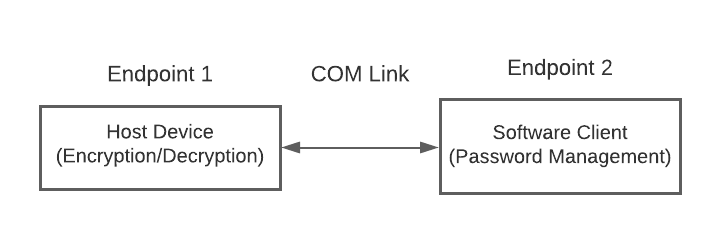
\includegraphics[width=0.65\columnwidth]{Figures/Fig_47.png}
\caption{Communication endpoints}
\label{fig:gantt}
\end{figure}



\subsection{Motivation}

Authentication of users using the system is important and two levels of authentication are required. The first is at the software client end to ensure that the end user is authorized to use the SSO system. This could be through a password verification step via a browser extension or the presence of key file within the users home directory for example. It should be noted that connection of the USB host device itself could be regarded as an authentication step as access to password storage is not possible without host attachment and it is assumed that only the legitimate user of the password manager has access to the USB device. 

The second authentication requirement is at the online account/service level. As part of the SSO capability of the end system a method of automatically submitting the required credentials and performing account sign on is required. 

Password managers may also have password generation capability. It should be noted that the rough goal of SSO is to allow a user to sign into any of their accounts using a single credential pair (i.e the password of the password manager for example). However for existing online accounts an option to add an existing credential pair could also be added. This has the limitation that the strength of the SSO credential relies on user supplied data rather than through a generator which may result in insecure passwords. However for a local SSO client, there is no straightforward method of changing the password of an online account. 



\subsection{Plan of development}

This paper consists of a literature review, followed by a high level and detailed design of the overall system. Next various experimentation will be conducted to evaluate the key security objectives. Finally results and conclusions will be drawn as well as proposals for future work on this topic.

For the literature review, this paper will review key concepts regarding SSO and password managers. Various exploitation vectors that lead to password compromise will then be investigated. Finally various encryption standards will be explored in order to ensure the secure storage of user credentials.

The design section of the paper follows and is expected to meet the key user requirements identified in section 6.1 (Table 7).
  
  
In the design section the various stages of prototype development will follow, starting with a high level representation of the respective hardware and software components and then progressing into physical designs that can be tested using the ATP (Acceptance Test Protocol) methodology. Various constraints around the development of the respective software and hardware exist including:

\begin{itemize}
  \item Time of implementation.
  \item Access to hardware and software components.
  \item Hardware limitations (such as clock speed).
  \end{itemize}
  
  
  Finally an attack surface analysis of the overall system will follow by investigating likely attack vectors and ranking their severity or potential impact. Both hardware and software exploitation techniques will be explored in an attempt to compromise the end system and retrieve sensitive credentials.
  
  Overall the total time spent on the project is divided into multiple phases (6) and is represented by the Gantt chart shown in Figure 1.2
  
\begin{figure}[H]
\centering
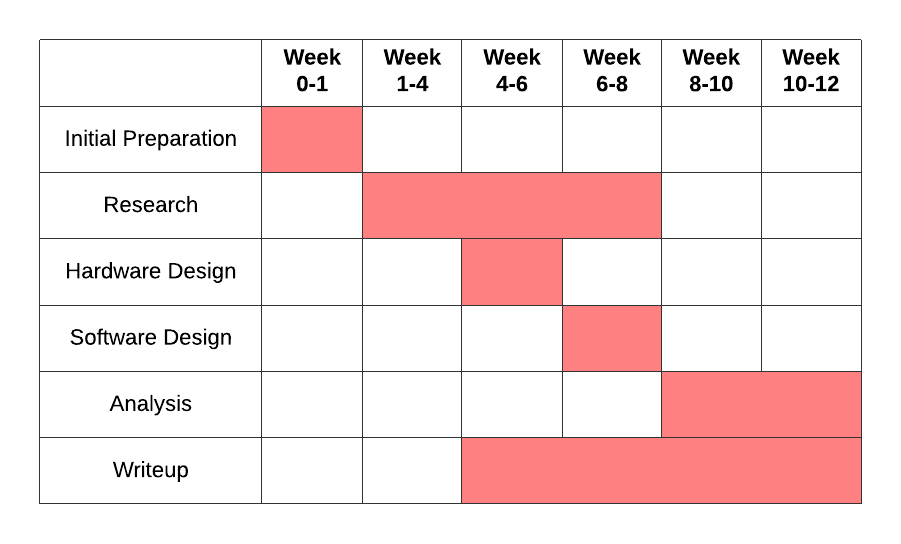
\includegraphics[width=0.8\columnwidth]{Figures/Fig_72.png}
\caption{Gantt chart showing division of work}
\label{fig:gantt}
\end{figure}

  As can be observed, weeks 0-1 constitute the preparation phase where the basic latex format for the report as well as additional materials are developed to support the rest of the project. The ordering of components for the project is also ideally to take place in the first week to ensure a timely hardware and software design phase.
  
  Next the research phase follows and is a critical component of the project and spans a total of 7 weeks (week 1-8). Here research is gathered to form part of the literature review that will accompany the report, additionally an investigation into possible hardware and software architectures for the USB drive takes place as well as early developmental hardware design.
  
  The actual hardware (week 4-6) and software (week 6-8) design phases then follow where the schematics and code samples are developed towards a working prototype.
  
  Finally an attack analysis of the overall system through experimentation follows (week 8-12) as well as the actual report write-up (week 4-12).